\chapter{Quantum Entanglements, Part 1}

These notes follow Leonard Susskind's second lecture in the supplementary \emph{Quantum Entanglement} track, in an edition curated by LazyingArt LLC. The lecture does not begin with entanglement itself. It begins with a simpler and more urgent question: what kind of state space can possibly describe a system that always yields only two measurement outcomes, and yet can still be prepared in many different directions? We will follow that question in the order in which the lecture builds it, beginning with a classical bit, passing through a deliberately classical but ultimately false picture of spin detection, and then moving into the complex vector space of states, inner products, basis states, and finally observables as matrices.

\section{Classical Bits, Qubits, and the Spin Example}

Up to this point the discussion has lived in classical physics. In that setting the state space is a Boolean space: a collection of points, one point for each possible state, with classical logic governing propositions about those states. A classical bit is the simplest example. It has two possibilities and nothing in between.

We can draw that classical bit as an object with two distinct orientations, up and down. If it points up, that is one state. If it points down, that is another. There is no intermediate classical state between them. That is the sense in which a classical bit is a two-state system.

The quantum bit, or qubit, is different, and Susskind chooses the simplest nontrivial example: the spin of an electron. Before any formalism is introduced, he pauses over a source of confusion that runs through the whole lecture. There are two different notions of vector in play.

First there is the ordinary vector of Euclidean space: an arrow with length and direction. To keep the language under control, we will call this a \emph{spatial vector}. The electron carries such a spatial vector in the form of its magnetic moment. All electrons have the same magnitude of magnetic moment, but that magnetic moment may point in different directions.

Second there is the abstract vector that belongs to a vector space of states. That is not an arrow in space. It is a mathematical object, and quantum mechanics will force us to use it.

So already the lecture places us under a certain pressure. The electron looks as though it carries a spatial arrow that may point in any direction, but the measurement story we are heading toward will refuse to behave continuously. That is where the puzzle begins.

\section{The Classical Preparation-and-Detection Story, and Why It Fails}

To sharpen the puzzle, the lecture first tells the wrong story on purpose. We remain classical for the moment.

Think of the electron as a tiny bar magnet with a north pole and a south pole. If we place it in a strong external magnetic field, its magnetic moment will not instantly snap into alignment. In a frictionless picture it precesses around the field, radiates away energy, and eventually settles into the lowest-energy orientation. This provides a classical model of \emph{preparation}: by choosing the direction of the external field, we choose the final direction of the electron's magnetic moment.

The same setup suggests a classical model of \emph{detection}. Put the electron into a known magnetic field and let it radiate as it relaxes. If the initial angle relative to the field is small, only a little energy is emitted. If the electron begins horizontal, more energy is emitted. If it begins anti-aligned, the emitted energy is maximal. In that classical picture, the readout is a continuous function of angle.

The schematic below keeps the lecture's experimental intuition while suppressing irrelevant detail.

\begin{figure}[h]
\centering
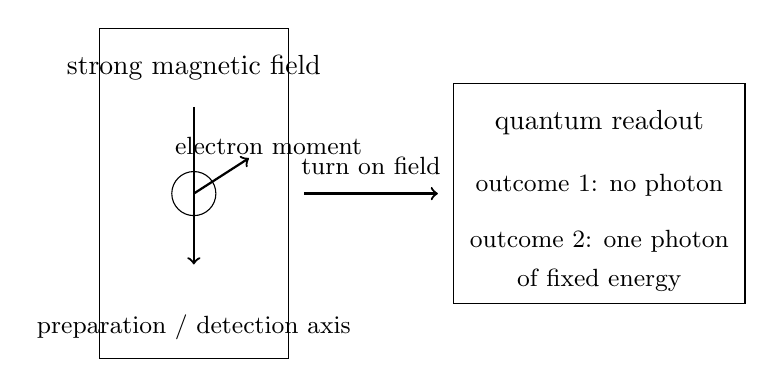
\begin{tikzpicture}[scale=1.0]
\draw (-0.2,0) rectangle (2.2,4.2);
\draw (1,3.7) node {strong magnetic field};
\draw[thick,->] (1,3.2) -- (1,1.2);
\draw (1,2.1) circle (0.28);
\draw[thick,->] (1,2.1) -- (1.7,2.55);
\draw (1.95,2.7) node {\small electron moment};
\draw (1,0.4) node {\small preparation / detection axis};

\draw (4.3,0.7) rectangle (8.0,3.5);
\draw (6.15,3.0) node {quantum readout};
\draw (6.15,2.2) node {\small outcome 1: no photon};
\draw (6.15,1.5) node {\small outcome 2: one photon};
\draw (6.15,1.0) node {\small of fixed energy};
\draw[->,thick] (2.4,2.1) -- (4.1,2.1);
\draw (3.25,2.45) node {\small turn on field};
\end{tikzpicture}
\end{figure}

If we wanted to summarize the false classical story mathematically, we would only say this:

\begin{remark}
In the classical picture the emitted energy is a continuous function of the initial angle relative to the magnetic field. The lecture does \emph{not} derive an explicit formula, and we should not insert one here.
\end{remark}

The lecture even sketches the qualitative graph one would expect classically.

\begin{figure}[h]
\centering
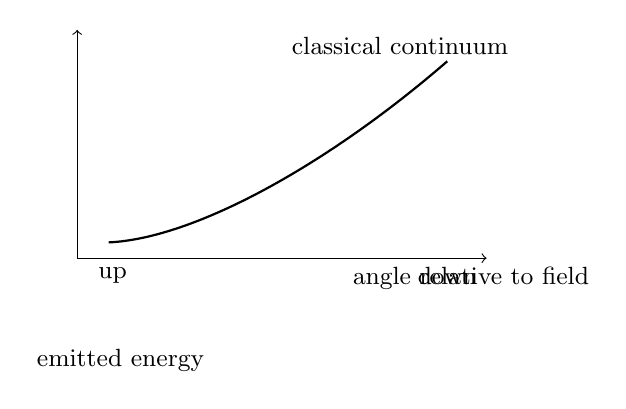
\begin{tikzpicture}[scale=1.0]
\draw[->] (0,0) -- (5.2,0);
\draw[->] (0,0) -- (0,2.9);
\draw (5.0,-0.25) node {\small angle relative to field};
\draw[rotate=90] (-1.3,-0.55) node {\small emitted energy};
\draw[thick] (0.4,0.2) .. controls (1.5,0.25) and (3.2,1.2) .. (4.7,2.5);
\draw (0.45,-0.22) node {\small up};
\draw (4.7,-0.22) node {\small down};
\draw (4.1,2.7) node {\small classical continuum};
\end{tikzpicture}
\end{figure}

But this whole story is wrong for a real electron. That is the first decisive pivot of the lecture.

For a genuine electron, once the magnetic field is turned on, only two outcomes occur:
\begin{itemize}
\item either no photon is emitted,
\item or one photon of a definite energy is emitted, namely the energy corresponding to the jump from the down state to the up state.
\end{itemize}

There is no continuum of possible emitted energies. The detector never reports a little bit of up, or mostly up, or almost down. It reports one of two outcomes.

What changes from one preparation to another is not the list of possible detector values. What changes is the probability distribution over those two values. If the electron is prepared vertically upward and measured in the same up-down device, the probability of emitting a photon is zero. If it is prepared vertically downward and then measured, that probability is one. If it is prepared horizontally and then measured in the vertical device, the probabilities are
\begin{equation}
P(\text{one photon})=\frac{1}{2},
\qquad
P(\text{no photon})=\frac{1}{2}.
\end{equation}

\subsection{Question \& Answer}

The lecture naturally raises the following question.

\paragraph{Question.} If the electron can be prepared in arbitrary directions, why does the up-down detector return only up or down?

\paragraph{Answer.} Because the preparation direction does not create new detector outcomes. It changes only the probabilities of the two outcomes available to that particular detector. A vertical detector always asks a binary question: up or down. What survives from the original preparation is a probability distribution, not a third detector value in between.

This point must be understood operationally. A single run does not reveal a probability distribution. To determine that distribution one must repeat the full prepare-and-measure cycle many times. Moreover, once a measurement has found the electron up, repeating the same measurement immediately afterward yields up again. The original preparation has no further role in that run. The experiment has fixed the state relative to that detector.

\section{From the Puzzle to a Complex Vector Space of States}

At this stage the lecture makes its central mathematical move. The state of a qubit is not described by two Boolean points. A two-point set cannot represent the fact that the detector has only two outcomes while the preparation can vary continuously. We need a different kind of state space.

Susskind chooses the minimum algebra needed to build that space: complex numbers.

A complex number is formed from two real numbers \(a\) and \(b\) together with the imaginary unit \(i\), defined by
\begin{equation}
i^2=-1.
\end{equation}
We write
\begin{equation}
z=a+ib,
\qquad
z^*=a-ib,
\end{equation}
where \(z^*\) is the complex conjugate of \(z\).

The board picture from the lecture's complex-number interlude belongs here, where the algebra is first being assembled for later physical use.

\begin{figure}[h]
\centering

\includegraphics[width=0.58\textwidth]{lecture_02_figure_02.png}
\end{figure}

A useful worked example is the product of a complex number with its conjugate:
\begin{align}
z^*z
&=(a-ib)(a+ib) \\
&=a^2+iab-iab-(ib)^2 \\
&=a^2+b^2.
\end{align}
The cross terms cancel, and because \(a\) and \(b\) are real, \(z^*z\) is real and nonnegative. This is exactly the pattern that will later make probabilities possible.

\begin{definition}
A complex vector space, in the sense needed for this lecture, is a collection of objects that can be added to one another and multiplied by complex numbers, with the result still lying in the same collection.
\end{definition}

The simplest example is the set of complex numbers itself. A more useful example is the set of column vectors with complex entries. If
\[
A \leftrightarrow \begin{pmatrix}A_1\\A_2\\A_3\end{pmatrix},
\]
then multiplication by a complex number \(c\) and addition of vectors are defined componentwise:
\begin{equation}
c\begin{pmatrix}A_1\\A_2\\A_3\end{pmatrix}
=
\begin{pmatrix}cA_1\\cA_2\\cA_3\end{pmatrix},
\end{equation}
and
\begin{equation}
\begin{pmatrix}A_1\\A_2\\A_3\end{pmatrix}
+
\begin{pmatrix}B_1\\B_2\\B_3\end{pmatrix}
=
\begin{pmatrix}A_1+B_1\\A_2+B_2\\A_3+B_3\end{pmatrix}.
\end{equation}

The qubit will live in the next simplest case: a two-dimensional complex vector space.

\section{Column Vectors, Bras, Kets, and the Inner Product}

The lecture now turns the abstract vector space into a practical notation. A state vector is written as a ket,
\[
|a\rangle \leftrightarrow \begin{pmatrix}a_1\\a_2\end{pmatrix}.
\]
Its conjugate partner is written as a bra,
\[
\langle a| \leftrightarrow \begin{pmatrix}a_1^* & a_2^*\end{pmatrix}.
\]
The star is not written on the bra symbol itself; it is implicit in turning the ket into its conjugate row.

This is the point at which the lecture deliberately keeps the formalism minimal. We are not being given the most general abstract definition of an inner product. We are being given the rule we need.

If
\[
|a\rangle \leftrightarrow \begin{pmatrix}a_1\\a_2\end{pmatrix},
\qquad
\langle b| \leftrightarrow \begin{pmatrix}b_1^* & b_2^*\end{pmatrix},
\]
then the inner product is
\begin{equation}
\langle b|a\rangle = b_1^*a_1+b_2^*a_2.
\end{equation}

When we take the inner product of a vector with itself, we obtain
\begin{equation}
\langle a|a\rangle = a_1^*a_1+a_2^*a_2.
\end{equation}
Each term is of the form \(z^*z\), so each term is real and nonnegative. Therefore \(\langle a|a\rangle\) is also real and nonnegative.

\begin{remark}
The lecture interprets \(\langle a|a\rangle\) as the square of the size of the vector. That is the quantity that will be set equal to \(1\) for physical states.
\end{remark}

Already one sees the shape of quantum mechanics emerging. Complex numbers are not decorative. Conjugation and the inner product are exactly what allow amplitudes to give positive probabilities.

\section{Up and Down as an Orthogonal Basis of States}

Having built the formal machinery, the lecture returns to the electron itself. We select two basis states, the states that an up-down detector can actually report, and denote them by
\[
|+\rangle \qquad \text{and} \qquad |-\rangle.
\]
In the chosen basis they are represented by the canonical columns
\begin{equation}
|+\rangle \leftrightarrow \begin{pmatrix}1\\0\end{pmatrix},
\qquad
|-\rangle \leftrightarrow \begin{pmatrix}0\\1\end{pmatrix}.
\end{equation}

The board snapshot below preserves the lecture's basis-fixing moment.

\begin{figure}[h]
\centering

\includegraphics[width=0.62\textwidth]{lecture_02_figure_04.png}
\end{figure}

A general qubit state is then a linear combination of these two basis states:
\begin{equation}
|\psi\rangle = a_+|+\rangle + a_-|-\rangle.
\end{equation}
In column-vector form this is
\begin{equation}
|\psi\rangle \leftrightarrow \begin{pmatrix}a_+\\a_-\end{pmatrix}.
\end{equation}
Indeed,
\[
a_+|+\rangle \leftrightarrow \begin{pmatrix}a_+\\0\end{pmatrix},
\qquad
a_-|-\rangle \leftrightarrow \begin{pmatrix}0\\a_-\end{pmatrix},
\]
and adding them gives the full state.

The lecture's board layout for this step is worth preserving.

\begin{figure}[h]
\centering

\includegraphics[width=0.68\textwidth]{lecture_02_figure_03.png}
\end{figure}

The coefficients are not themselves probabilities. Their squared magnitudes are:
\begin{equation}
P(+)=a_+^*a_+=|a_+|^2,
\qquad
P(-)=a_-^*a_-=|a_-|^2.
\end{equation}
Since the probabilities must add to one, physical states are normalized:
\begin{equation}
|a_+|^2+|a_-|^2=1.
\end{equation}
Equivalently,
\begin{equation}
\langle \psi|\psi\rangle = 1.
\end{equation}

The basis vectors are orthonormal:
\begin{align}
\langle +|+\rangle &= 1, &
\langle -|-\rangle &= 1, \\
\langle +|-\rangle &= 0, &
\langle -|+\rangle &= 0.
\end{align}
Thus the up and down states are represented by orthogonal vectors in the state space.

\paragraph{Worked example.}
The lecture makes an instructive stumble here and immediately corrects it. If we try
\[
\begin{pmatrix}1\\1\end{pmatrix},
\]
we have written something that is not yet a physical state, because its norm-squared is \(1+1=2\). To normalize it, we divide by \(\sqrt{2}\):
\begin{equation}
\frac{1}{\sqrt{2}}\begin{pmatrix}1\\1\end{pmatrix}.
\end{equation}
Now
\[
P(+)=\frac{1}{2},
\qquad
P(-)=\frac{1}{2}.
\]
This is the lecture's first explicit example of a state that is neither pure up nor pure down. It is one of the states associated with a horizontal preparation.

So the new mathematics resolves the original tension in a very specific way. The detector still returns only up or down. But the electron can occupy other physical states because the state space contains linear combinations of the up and down basis vectors.

\section{What the State Vector Does and Does Not Encode}

After the break, the lecture returns to a likely source of confusion. The spatial vector carried by the electron and the abstract state vector of the qubit are related, but not simply related.

A spatial vector in ordinary space has three real components. A two-component state vector,
\[
\begin{pmatrix}a_+\\a_-\end{pmatrix},
\]
has two complex components, which at first sight means four real numbers. So the two objects are plainly not the same kind of thing.

This is already enough to warn us away from naive identifications. We should not imagine that the two entries of the state vector are just the \(x\)- and \(y\)-components of a little arrow in space. They are amplitudes in an abstract vector space of states. The precise bridge back to spatial direction will come later.

There is also a second point of notation that the lecture insists on: the symbols \(+\) and \(-\) in \(|+\rangle\) and \(|-\rangle\) are labels, not arithmetic signs. They label the two basis states selected by the up-down measurement.

\subsection{Question \& Answer}

\paragraph{Question.} Is \(-|+\rangle\) the same thing as \(|-\rangle\)?

\paragraph{Answer.} No. The symbol \(-\) in \(|-\rangle\) is part of the label of a basis state. It does not mean minus one times the plus state. On the other hand, \(-|+\rangle\) is a perfectly legitimate scalar multiple of \(|+\rangle\), and it represents the same physics as \(|+\rangle\) so far as probabilities are concerned. More generally, multiplying a state by any complex number of magnitude one does not change the physical state. But changing a relative sign inside a superposition may change the state. Thus
\[
|\psi\rangle = a_+|+\rangle + a_-|-\rangle
\]
and
\[
|\psi'\rangle = a_+|+\rangle - a_-|-\rangle
\]
need not represent the same physics.

The lecture does not yet develop the full geometry of phase. It only establishes the minimum point we need: overall phase is physically inessential, while relative phase inside a superposition can matter.

One further structural point is also emphasized. The dimension of the state space is read off experimentally. In the present case the up-down detector has two possible outcomes, and that is why the spin of an electron is described, at this stage, by a two-dimensional complex vector space.

\section{From Classical Observables to Quantum Matrices}

So far we have discussed states. Now the lecture turns to the things one measures.

In classical mechanics, if the set of possible states is a collection of points labeled by \(n\), then an observable is simply a real-valued function on those points:
\[
f_n.
\]
If the system is definitely in state \(n\), the observable has value \(f_n\). If instead there is only a probability distribution \(p_n\) over states, then the average value of the observable is
\begin{equation}
\langle f\rangle = \sum_n p_n f_n.
\end{equation}

This is reviewed first in a purely classical spirit. For a two-outcome observable taking the values \(+1\) and \(-1\), with probabilities \(p_+\) and \(p_-\), the average is
\begin{equation}
\langle f\rangle = p_+ - p_-.
\end{equation}
The lecture pauses over an important conceptual point: the average value need not itself be a possible outcome. If \(p_+=p_-=\frac{1}{2}\), then the average is zero, even though zero is not one of the detector values.

A special observable is the indicator function that is equal to \(1\) on one state and \(0\) on all the others. In that case the average is just the probability of that state. Thus knowledge of all average values is enough, in principle, to reconstruct probability distributions.

Quantum mechanics now changes the mathematical representation of observables. They are no longer just functions on state points. They become linear operators, represented in the present finite-dimensional setting by matrices.

The board snapshot below marks this transition very clearly: abstract operator notation above, explicit matrix action below.

\begin{figure}[h]
\centering

\includegraphics[width=0.66\textwidth]{lecture_02_figure_05.png}
\end{figure}

If
\[
M=\begin{pmatrix}m_{11}&m_{12}\\m_{21}&m_{22}\end{pmatrix},
\qquad
|a\rangle=\begin{pmatrix}a_1\\a_2\end{pmatrix},
\]
then
\begin{equation}
M|a\rangle = |a'\rangle,
\end{equation}
with component rule
\begin{equation}
\begin{pmatrix}
m_{11} & m_{12} \\
m_{21} & m_{22}
\end{pmatrix}
\begin{pmatrix}
a_1 \\
a_2
\end{pmatrix}
=
\begin{pmatrix}
m_{11}a_1+m_{12}a_2 \\
m_{21}a_1+m_{22}a_2
\end{pmatrix}.
\end{equation}

In the lecture these matrices are first motivated geometrically, using an ordinary two-dimensional real vector space. A few examples are enough to show what matrices do:
\begin{itemize}
\item
\[
\begin{pmatrix}
2 & 0 \\
0 & 2
\end{pmatrix}
\]
doubles every vector.

\item
\[
\begin{pmatrix}
1 & 0 \\
0 & 2
\end{pmatrix}
\]
stretches only the \(y\)-component.

\item
\[
\begin{pmatrix}
0 & 1 \\
1 & 0
\end{pmatrix}
\]
interchanges \(x\) and \(y\), and therefore reflects the plane across the diagonal \(x=y\).

\item
\[
\begin{pmatrix}
0 & 1 \\
-1 & 0
\end{pmatrix}
\]
rotates the plane by \(90^\circ\) in the convention discussed on the board.
\end{itemize}

The point of these examples is not that the electron literally lives in this plane. The point is that matrices represent linear transformations of vector spaces.

The special class of matrices relevant for observables is the class of Hermitian matrices.

\begin{definition}
A matrix \(M\) is Hermitian if
\begin{equation}
M_{ij}=M_{ji}^*.
\end{equation}
\end{definition}

Immediately one consequence follows: setting \(i=j\) gives
\[
M_{ii}=M_{ii}^*,
\]
so the diagonal elements are real. Off-diagonal elements come in complex-conjugate pairs.

This is the lecture's closing mathematical postulate for the next step:
\begin{remark}
Hermitian matrices are the quantum representatives of observables, just as real-valued functions on state points are the classical representatives of observables.
\end{remark}

A final preview is given but not developed here. If one wants to \emph{do} something to the state, rather than merely represent a measurable quantity, one is led to unitary operators. The only fact stated at this stage is that unitary operators preserve the length of vectors. Their full role belongs to the next lecture.

\section{Summary}

The lecture has now established the mathematical entrance to quantum mechanics. A classical bit is a two-point Boolean system. The spin of an electron refuses to fit that description: it can be prepared in many directions, but a fixed detector returns only two outcomes. That tension drives us away from a set of states and into a complex vector space of states.

Within that space we introduced complex numbers, conjugation, column vectors, bras, kets, and the inner product. We chose the orthonormal basis \(|+\rangle\) and \(|-\rangle\), wrote a general qubit state as
\[
|\psi\rangle=a_+|+\rangle+a_-|-\rangle,
\]
and interpreted \(|a_+|^2\) and \(|a_-|^2\) as the probabilities of the two detector outcomes. We then shifted from states to observables, reviewed the classical average
\[
\langle f\rangle=\sum_n p_n f_n,
\]
and replaced classical observable-functions by quantum matrices, with Hermitian matrices singled out as the measurable ones.

This is exactly the amount of mathematics the lecture insists upon before one can honestly discuss entanglement. Once these notions are secure, the connection between spin components, matrices, and real directions in space can be developed without sleight of hand.